\documentclass[a4paper, 9pt]{article}
\usepackage{geometry}
\geometry{a4paper, margin=1.5cm}
%\usepackage{tgcursor}
\usepackage{multicol}
\usepackage{varwidth}
\usepackage[italian]{babel}
\usepackage{tabto}
\usepackage{subcaption}
\usepackage{graphicx}
\usepackage{wrapfig}
\usepackage{amsmath}
\usepackage[dvipsnames, table]{xcolor}
\usepackage{floatflt}
\usepackage{float}
\usepackage{hyperref}
\usepackage{listings}
\usepackage{xcolor}
\usepackage{tabularx}
\usepackage[most]{tcolorbox}
\usepackage{epigraph}
\tcbuselibrary{raster}
\usepackage{fontawesome5} 
\usepackage{enumitem}
\usepackage{fancyhdr}
\usepackage{extramarks}


\definecolor{codegreen}{rgb}{0.0,0.6,0.0}
\definecolor{codegray}{rgb}{0.5,0.5,0.5}
\definecolor{codeblue}{RGB}{16, 16, 148}
\definecolor{codepurple}{rgb}{0.58,0,0.82}
\definecolor{backcolour}{rgb}{0.95,0.95,0.92}
\definecolor{coloresempio}{RGB}{207, 221, 244}

\hypersetup{
    colorlinks=true,
    linkcolor=blue,
    filecolor=magenta,      
    urlcolor=cyan,
    pdftitle={Overleaf Example},
    pdfpagemode=FullScreen,
    }
\urlstyle{same}



\newtcolorbox[auto counter, number within=section]{esempio}[2][]{
    enhanced,                          % Abilita grafiche avanzate
    breakable,
    title={Esempio \thetcbcounter: #2}, % Titolo automatico
    colback=coloresempio,                     % Colore del corpo del box
    colframe=NavyBlue,                 % Colore del bordo e dell'header
    coltitle=white,                    % Colore del testo del titolo
    fonttitle=\bfseries,               % Titolo in grassetto
    boxrule=1pt,                       % Spessore del bordo esterno
    arc=4pt,                           % Arrotondamento angoli
    toptitle=2pt,                      % Spazio sopra il titolo nell'header
    bottomtitle=2pt,                   % Spazio sotto il titolo nell'header
    left=10pt,                          % Padding interno sinistro
    right=10pt,                         % Padding interno destro
    #1                                 % Permette personalizzazioni extra
}

\lstdefinestyle{mystyle}{
    backgroundcolor=\color{backcolour},   
    commentstyle=\color{codegreen},
    keywordstyle=\color{magenta}\bfseries,
    % --- SECONDO GRUPPO DI KEYWORDS / TIPI (Blu) ---
    ndkeywordstyle=\color{codeblue}\bfseries,
    % --- STILE DI COMMENTI E STRINGHE ---
    commentstyle=\color{codegreen}\itshape,
    stringstyle=\color{codepurple},
        % --- TRUCCO PER COLORARE I NUMERI COINVOLTI NEL CODICE (Viola) ---
        literate=*
            {0}{{\color{codepurple}0}}{1}
            {1}{{\color{codepurple}1}}{1}
            {2}{{\color{codepurple}2}}{1}
            {3}{{\color{codepurple}3}}{1}
            {4}{{\color{codepurple}4}}{1}
            {5}{{\color{codepurple}5}}{1}
            {6}{{\color{codepurple}6}}{1}
            {7}{{\color{codepurple}7}}{1}
            {8}{{\color{codepurple}8}}{1}
            {9}{{\color{codepurple}9}}{1},
    numberstyle=\tiny\color{codegray},
    basicstyle=\ttfamily\footnotesize,
    escapeinside={(*}{*)}, % Definisce (* e *) come delimitatori per uscire dal codice,
    breakatwhitespace=false,         
    breaklines=true,                 
    captionpos=b,                    
    keepspaces=true,                 
    numbers=left,                          
    firstnumber=1,
    numbersep=5pt,                  
    showspaces=false,                
    showstringspaces=false,
    showtabs=false,                  
    tabsize=2,
    frame=single % adds a frame around the code
}

\lstset{style=mystyle}

\newcounter{nalg}[section] % defines algorithm counter for chapter-level
\renewcommand{\thenalg}{\thesection .\arabic{nalg}} %defines appearance of the algorithm counter
\DeclareCaptionLabelFormat{algocaption}{Algoritmo \thenalg} % defines a new caption label as Algorithm x.y

\lstnewenvironment{myalgo}[1][] %defines the algorithm listing environment
{   
    \refstepcounter{nalg} %increments algorithm number
    \captionsetup{labelformat=algocaption,labelsep=colon} %defines the caption setup for: it ises label format as the declared caption label above and makes label and caption text to be separated by a ':'
    \lstset{ %this is the stype
        mathescape=true,
        frame=tB,
        numbers=left, 
        numberstyle=\tiny,
        basicstyle=\scriptsize\ttfamily, 
        keywordstyle=\color{black}\bfseries\em,
        keywords={,INPUT, OUTPUT, return, datatype, function, in, if, else, foreach, while, begin, end, then, nil, for, all, continue, break, do, True, False, repeat, until,} %add the keywords you want, or load a language 
        ndkeywords={Basic, Block, float, double, char, void, bool, Matrix, array, successors},
        ndkeywordstyle=\color{codeblue}\bfseries,
        numbers=left,
        xleftmargin=.04\textwidth,
        #1 % this is to add specific settings to an usage of this environment (for instnce, the caption and referable label)
    }
}
{}


% --- PALETTE COLORI LABORATORIO ---
\definecolor{LabNavy}{HTML}{002147}
\definecolor{LabBlue}{HTML}{005EB8}
\definecolor{ConsoleBG}{HTML}{1A1A1A}


% 2. AMBIENTE CONSOLE (Per comandi Cisco/Linux)
\newtcolorbox{console}[1][]{
    enhanced,
    colback=ConsoleBG,
    colupper=green!80!white,
    fontupper=\ttfamily\small,
    sharp corners,
    boxrule=0pt,
    left=3mm,
    title={\tiny \faTerminal\quad CONSOLE},
    coltitle=gray!50,
    fonttitle=\ttfamily\scriptsize,
    attach boxed title to top right={yshift=-1.5mm, xshift=-2mm},
    boxed title style={colback=ConsoleBG, boxrule=0pt},
    #1
}

% 4. AMBIENTE NOTA TECNICA (Stile Warning/Attenzione)
\newtcolorbox{notatecnica}[1][]{
    enhanced,
    breakable,
    title={\faExclamationTriangle\quad NOTA TECNICA},
    fonttitle=\bfseries\sffamily,
    coltitle=orange!60!black,    % Colore del testo del titolo scuro per leggibilità
    colback=yellow!10,           % Sfondo giallino/arancio chiaro
    colframe=orange,             % Bordo arancione
    sharp corners,               % Mantiene lo stile squadrato degli altri box
    boxrule=1pt,                 % Spessore del bordo
    top=3mm, bottom=3mm,
    left=4mm, right=4mm,
    before skip=10pt,
    after skip=10pt,
    #1                           % Permette modifiche extra al volo
}

\newtcolorbox{boxsemplice}[1][]{
    enhanced,
    breakable,
    colback=gray!5,       % Sfondo grigio chiarissimo
    colframe=gray!40,     % Bordo grigio medio
    boxrule=0.5pt,        % Bordo sottile
    sharp corners,        % Angoli vivi, stile pulito
    left=3mm, right=3mm,  % Margini interni
    top=3mm, bottom=3mm,
    before skip=6pt,      % Spazio prima del box
    after skip=6pt,       % Spazio dopo il box
    #1                    % Permette modifiche al volo
}





% --- AMBIENTE PERSONALIZZATO PER LE TABELLE DFA ---
\newtcolorbox{tabelladfa}[1]{%
    enhanced,
    breakable,
    colframe=NavyBlue,       % Usa lo stesso blu scuro dei tuoi laboratori
    colback=gray!5,          % Sfondo interno del box bianco
    fonttitle=\bfseries\sffamily,
    coltitle=white,
    title={#1},             % Il titolo della tabella viene passato come argomento
    attach boxed title to top left={yshift=-2mm, xshift=5mm},
    boxed title style={colback=NavyBlue, sharp corners, boxrule=0pt},
    sharp corners,
    boxrule=1pt,
    top=4mm, bottom=2mm, left=2mm, right=2mm,
    before skip=0.8cm, after skip=0.8cm
}

\newtcolorbox{frameworkdfa}[1]{%
    enhanced,
    breakable,
    colframe=NavyBlue,        % Bordo blu scuro elegante
    colback=gray!5,           % Sfondo grigio chiarissimo per le righe
    fonttitle=\bfseries\sffamily,
    coltitle=white,
    title={Framework: #1},     % Prende il nome del problema come titolo
    attach boxed title to top left={yshift=-2mm, xshift=5mm},
    boxed title style={colback=NavyBlue, sharp corners, boxrule=0pt},
    sharp corners,
    boxrule=1pt,
    top=4mm, bottom=2mm, left=2mm, right=2mm,
    before skip=0.8cm, after skip=0.8cm
}

%
% Basic Document Settings
%

\topmargin=-0.45in
\evensidemargin=0in
\oddsidemargin=0in
\textwidth=6.5in
\textheight=9.0in
\headsep=0.25in

\linespread{1.1}

\pagestyle{fancy}
\lhead{\hmwkAuthorName}
\chead{\hmwkTitle}
\rhead{\leftmark} % <- Questo mostrerà dinamicamente il nome del problema corrente!
\lfoot{}
\cfoot{\thepage}

\renewcommand\headrulewidth{0.4pt}
\renewcommand\footrulewidth{0.3pt}

\setlength\parindent{0pt}

\setcounter{secnumdepth}{1}

% Homework Details
%   - Title
%   - Due date
%   - Class
%   - Section/Time
%   - Instructor
%   - Author
%

\newcommand{\hmwkTitle}{Secondo Assignment}
\newcommand{\hmwkDueDate}{Giugno 2026}
\newcommand{\hmwkClass}{Linguaggi e Compilatori}
\newcommand{\hmwkClassTime}{Middle-end}
\newcommand{\hmwkAuthorName}{\textbf{Jeta Derveni}}

%
% Title Page
%

\title{
    \vspace{2in}
    \textmd{\textbf{\hmwkClass:\ \hmwkClassTime}}\\
    \normalsize\vspace{0.1in}\small{\hmwkDueDate}\\
    \vspace{0.5in}\Large{\textit{ \hmwkTitle}}
    \vspace{3in}
}

\author{\hmwkAuthorName}
\date{}

\renewcommand{\part}[1]{\textbf{\large Part \Alph{partCounter}}\stepcounter{partCounter}\\}

%
% Various Helper Commands
%

% Useful for algorithms
\newcommand{\alg}[1]{\textsc{\bfseries \footnotesize #1}}

% For derivatives
\newcommand{\deriv}[1]{\frac{\mathrm{d}}{\mathrm{d}x} (#1)}

% For partial derivatives
\newcommand{\pderiv}[2]{\frac{\partial}{\partial #1} (#2)}

% Integral dx
\newcommand{\dx}{\mathrm{d}x}

% Alias for the Solution section header
\newcommand{\solution}{\textbf{\large Solution}}



\begin{document}
\renewcommand{\labelenumii}{\arabic{enumi}.\arabic{enumii}}
\renewcommand{\labelenumiii}{\arabic{enumi}.\arabic{enumii}.\arabic{enumiii}}
\renewcommand{\labelenumiv}{\arabic{enumi}.\arabic{enumii}.\arabic{enumiii}.\arabic{enumiv}}
\newcommand{\chapsubhead}[1]{{\Large #1 \vspace{2ex}}}
\newcommand{\chaptype}[1]{{\Large \itshape (#1) \vspace{2ex}}}
\maketitle
\pagebreak

%\pagenumbering{roman}
%\tableofcontents
%\newpage
\pagenumbering{arabic}


\section{Very Busy Expressions}
\begin{figure}[H]
    \centering
    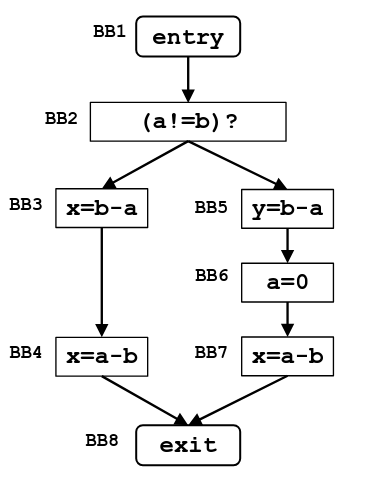
\includegraphics[width=.4\textwidth]{./img/img1.png}
\end{figure}
%Quelle che dovremmo analizzare sono le espressioni del programma, perciò gli insiemi IN[B] e OUT[B] conterranno le %espressioni. La direzione dell'analisi è backward, siccome i valori di uscita OUT[b] dipendono dai valori in entrata degli successori. Vogliamo capire cosa succede a un'espressione se dal punto p si va avanti percorrendo uno dei suoi successori. OUT[B] = intersezione INs per ogni successore . Per le condizioni di contorno, all'inizio del blocco di uscita, nessuna espressione può essere busy o può essere uccisa, quindi poniamo IN[EXIT]= empty. Siccome il meet operator è l'intersezione, inizializziamo IN[B] per ogni blocco all'insieme universo. In questo modo, ci assicuriamo che la soluzione converga sempre. (Se IN[B] = empty per ogni B, dovremmo fare in un certo punto out[b] = IN[SUC] INTERSEZIONE ..... CHE SONO TUTTE VUOTE E OUT[B] RISULTERÀ SEMPRE VUOTO.) La funzione di trasferimento: al punto di programma che coincide con l'inizio di un basic block B, le espressioni very busy sono quelle che vengono usate all'interno del blocco in esaminazione unite all'insieme di espressioni che raggiungono la fine del blocco tolte le espressioni che sono state uccise in seguito di una ridefinizione di un operando.
\begin{frameworkdfa}{Very Busy Expressions}
    \centering
    \begin{tabularx}{\textwidth}{>{\bfseries\sffamily}l | X}
        Domain & Insieme di espressioni \\
        \\
        \hline
        Direction & Backward: $$IN[B] = f_b(OUT[B])$$  $$OUT[B] = \cap IN[succ(B)]$$ \\
        \hline
        Transfer function & $IN[B] = USE[B] \cup (OUT[B] - KILL[B])$ \\
        \hline
        Meet Operation ($\wedge$) & Intersezione ($\cap$) \\
        \hline
        Boundary Condition & $IN[EXIT] = \emptyset$ \\
        \hline
        Initial interior points & $IN[B] = U$ \\
    \end{tabularx}
\end{frameworkdfa}
L'algoritmo iterativo per la soluzione del problema data-flow delle Very Busy Expressions è:
\begin{myalgo}[style=mystyle]
INPUT: CFG
OUTPUT: IN[B], OUT[B] $\forall$ Basic Block B 

//Boundary condition 
IN[EXIT] = $\emptyset$

//Initialization
foreach B other than Exit 
    IN[B] = $\mathcal{U}$
while(changes in IN[] occur){
    foreach B other than Exit {
        OUT[B] = $\cap$(IN[S]) $\forall$ successors S of B
        IN[B] = use$_B$ $\cup$ (OUT[B] - kill$_B$)
    }
}
\end{myalgo}
Prima di tutto si calcolano gli insiemi use$_B$ e kill$_B$, che rappresentano rispettivamente gli insiemi di espressioni che vengono usate ed espressioni che vengono uccise a causa della definizione di uno degli operandi all'interno del Basic Block B.$$kill\_B = \{x \odot  y \in \mathcal{U}| x \in defs_B \vee  y \in defs_B \}$$ 
\begin{itemize}
    \item BB8 è il blocco di uscita, quindi non usa e non uccide nessuna espressione. use$_8=\emptyset$ e kill$_8=\emptyset$
    \item BB4 use$_4=\{a-b\}$ e kill$_4=\emptyset$
    \item BB7 use$_7=\{a -b\}$ e kill$_7=\emptyset$
    \item BB3 use$_3=\{b -a\}$ e kill$_3=\emptyset$
    \item BB6 non usa nessuna espressione use$_6=\emptyset$ ma con la definizione della variabile $a$ uccide tutte le espressioni in cui $a$ è un operando kill$_6=\{a -b, b- a\}$
    \item BB5 use$_5=\{b -a\}$ e kill$_5=\emptyset$
    \item BB2 use$_2=\emptyset$ e kill$_2=\emptyset$
    \item BB1 (entry) use$_1=\emptyset$ e kill$_1=\emptyset$
\end{itemize}
L'algoritmo si applica fino a convergenza. Dopo la seconda iterazione gli insiemi IN[B] non cambiano più. 
$$OUT[B] = \cap(IN[S]) \forall \text{ successors S of B}$$
$$IN[B] = use_B \cup (OUT[B] - kill_B)$$
\begin{tabelladfa}{Iterazioni}
    \centering
    \small % Rimpicciolisce leggermente il testo per far stare tutto comodamente
    \renewcommand{\arraystretch}{1.3} % Aumenta leggermente l'altezza delle righe come nell'immagine
    
    \begin{tabularx}{\textwidth}{>{\bfseries}l | X | X | X | X}
        
        % Prima riga di intestazione: raggruppa le colonne a due a due
        \rowcolor{NavyBlue!40} % Colore di sfondo opzionale per la prima riga intestazione
        & \multicolumn{2}{c|}{\textbf{Iterazione 1}} & \multicolumn{2}{c}{\textbf{Iterazione 2}} \\
        
        % Seconda riga di intestazione: specifica IN e OUT
        \rowcolor{LabBlue!20}
        \textbf{Blocco} & \hfil $IN[B]$ \hfil & \hfil $OUT[B]$ \hfil & \hfil $IN[B]$ \hfil & \hfil $OUT[B]$ \hfil  \\
        \hline
        
        % Dati della tabella
        BB1 & $ \{b-a\}$ & $ \{b-a\} $ & $ \{b-a\}$ & $ \{b-a\} $   \\
        \hline
        BB2 & $\{b-a\}$&$\{b-a\}$ & $\{b-a\}$&$\{b-a\}$    \\
        \hline
        BB3 & $\{a - b,b-a\}$& $\{a-b\}$ & $\{a - b,b-a\}$& $\{a-b\}$\\
        \hline
        BB4 &$\{a - b\}$ & $\emptyset$ &$\{a - b\}$ & $\emptyset$  \\
        \hline
        BB5 & $\{b-a\}$& $\emptyset$ & $\{b-a\}$& $\emptyset$   \\
        \hline
        BB6 &$\emptyset$ & $\{a-b\}$ &$\emptyset$ & $\{a-b\}$ \\
        \hline
        BB7 &$\{a - b\}$ & $\emptyset$ &$\{a - b\}$ & $\emptyset$  \\
        \hline
        BB8 &$\emptyset$ & $\emptyset$ &$\emptyset$ & $\emptyset$   \\
    \end{tabularx}

\end{tabelladfa}
\pagebreak
\section{Dominator Analysis}
%pagina 137 libro
\begin{figure}[H]
    \centering
    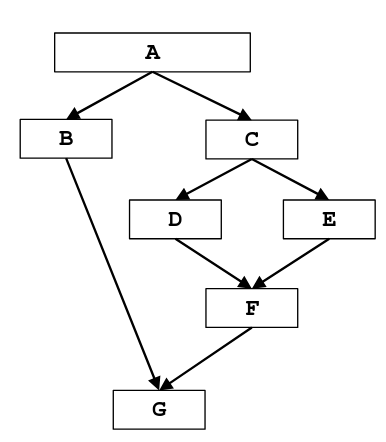
\includegraphics[width=.5\textwidth]{./img/img2.png}
\end{figure}
L'insieme dei nodi dominanti del basic block B, scritta come DOM[B], coincide con l'insieme OUT[B] del problema data-flow. Per coerenza con la trattazione generale dell'analisi data-flow, si è scelto di mantenere la notazione standard basata sugli insiemi IN[B] e OUT[B].
$$DOM[B] \equiv OUT[B]$$
\begin{frameworkdfa}{Dominator Analysis}
    \centering
    \begin{tabularx}{\textwidth}{>{\bfseries\sffamily}l | X}
        Domain & L'insieme potenza dei nodi del CFG \textrightarrow Basic Blocks\\
        \hline
        Direction & Forward $$IN[B] = \cap_{P \in pred(B)}OUT[P] $$ $$OUT[B] = f_B(IN[B]) $$\\
        \hline
        Transfer function & $OUT[B] = IN[B]\cup \{B\}$  \\
        \hline
        Meet Operation ($\wedge$) & Intersezione ($\cap$) \\
        \hline
        Boundary Condition & $OUT[ENTRY] = \{ENTRY\}$ \\
        \hline
        Initial interior points &  $OUT[B]=\mathcal{U}$ (l'insieme di tutti i nodi del CFG)\\
    \end{tabularx}
\end{frameworkdfa}
L'algoritmo iterativo per la soluzione della Dominator Analysis è:
\begin{myalgo}[style=mystyle]
INPUT: CFG
OUTPUT: IN[B], OUT[B] $\forall$ Basic Block B 

//Boundary condition 
OUT[ENTRY] = $\{ENTRY\}$

//Initialization
foreach B other than Entry 
    OUT[B] = $\mathcal{U}$
while(changes in OUT[] occur){
    foreach B other than Entry {
        IN[B] = $\cap_{P \in pred(B)}OUT[P]$
        OUT[B] = $IN[B]\cup \{B\}$
    }
}
\end{myalgo}


\begin{tabelladfa}{Iterazioni}
    \centering
    \small % Rimpicciolisce leggermente il testo per far stare tutto comodamente
    \renewcommand{\arraystretch}{1.3} % Aumenta leggermente l'altezza delle righe come nell'immagine
    
    \begin{tabularx}{\textwidth}{>{\bfseries}l | X | X | X | X}
        
        % Prima riga di intestazione: raggruppa le colonne a due a due
        \rowcolor{NavyBlue!40} % Colore di sfondo opzionale per la prima riga intestazione
        & \multicolumn{2}{c|}{\textbf{Iterazione 1}} & \multicolumn{2}{c}{\textbf{Iterazione 2}}  \\
        
        % Seconda riga di intestazione: specifica IN e OUT
        \rowcolor{LabBlue!20}
        \textbf{Blocco} & \hfil $IN[B]$ \hfil & \hfil $OUT[B]$ \hfil & \hfil $IN[B]$ \hfil & \hfil $OUT[B]$ \hfil\\
        \hline
        
        % Dati della tabella
        A & $\emptyset$ & $\{A\}$ & $\emptyset$& $\{A\}$  \\
        \hline
        B & $\{A\}$ & $\{A,B\}$ & $\{A\}$ & $\{A,B\}$\\
        \hline
        C &$\{A\}$ &$\{A,C\}$  &$\{A\}$ &$\{A,C\}$  \\
        \hline
        D &$\{A, C\}$ &$\{A,C,D\}$ &$\{A, C\}$ &$\{A,C,D\}$   \\
        \hline
        E & $\{A,C\}$&$\{A,C,E\}$  & $\{A,C\}$&$\{A,C,E\}$  \\
        \hline
        F & $\{A,C\}$&$\{A,C,F\}$ & $\{A,C\}$&$\{A,C,F\}$ \\
        \hline
        G &$\{A\}$ & $\{A,G\}$  &$\{A\}$ & $\{A,G\}$\\
    \end{tabularx}

\end{tabelladfa}
\pagebreak
\section{Constant Propagation}
\begin{figure}[H]
    \centering
    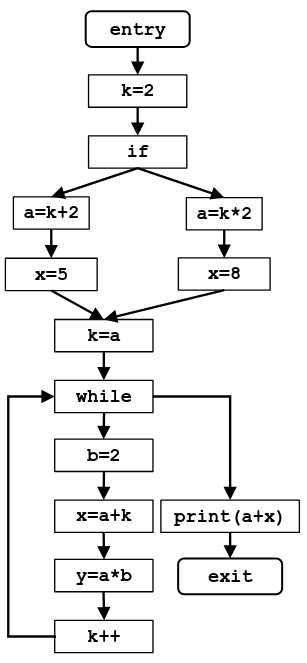
\includegraphics[width=.4\textwidth]{./img/img3.png}
    \caption{}
    \label{fig:fi3}
\end{figure}
\begin{frameworkdfa}{Constant Propagation}
    \centering
    \begin{tabularx}{\textwidth}{>{\bfseries\sffamily}l | X}
        Domain & Insieme di coppie di valori $\langle variabile , costante\rangle $  \\
        \hline
        Direction & Forward $$IN[B] = \cap_{P \in pred(B)}OUT[P] $$ $$OUT[B] = f_B(IN[B]) $$\\ \\
        \hline
        Transfer function & $OUT[B] = GEN[B] \cup (IN[B] \setminus KILL[B])$ \\
        \hline
        Meet Operation ($\wedge$) & Intersezione ($\cap$) \\
        \hline
        Boundary Condition & $OUT[ENTRY] = \emptyset$ \\
        \hline
        Initial interior points & $OUT[B] = \mathcal{U}$ (tutte le possibili coppie $\langle variabile,costante \rangle$)\\
    \end{tabularx}
\end{frameworkdfa}

\begin{myalgo}[style=mystyle]
INPUT: CFG
OUTPUT: IN[B], OUT[B] $\forall$ Basic Block B 

//Boundary condition 
OUT[ENTRY] = $\emptyset$

//Initialization
foreach B other than Entry 
    OUT[B] = $\mathcal{U}$
while(changes in OUT[] occur){
    foreach B other than Entry {
        IN[B] = $\cap_{P \in pred(B)}OUT[P]$
        OUT[B] = $GEN[B] \cup (IN[B] \setminus KILL[B])$
    }
}
\end{myalgo}
%$$gen_B = \{ \langle x,c rangle \in IN[B] | x è sovrascritto in B\}$$
%$$kill_B = \{ \langle x,c rangle \in IN[B] | x è sovrascritto in B\}$$
Nella tabella \ref{tab:iter3} viene mostrata l'esecuzione dell'algoritmo iterativo sul CFG di figura \ref{fig:fi3}. L'algoritmo si arresta dopo la terza iterazione, poiché gli insiemi IN[B] e OUT[B] calcolati coincidono esattamente con quelli dell'iterazione precedente. Ulteriori iterazioni non modificherebbero più la soluzione.\\
%Insiemi \texttt{gen$_B$} e \texttt{kill$_B$} per ogni Basic Block:
%\begin{itemize}
%    \item BB1 \textrightarrow gen$_1$=$\emptyset$ e kill$_1$=$\emptyset$
 %   \item BB2 \textrightarrow gen$_2$=$\{\langle k,2 \rangle\}$ e kill$_2$=$\emptyset$
  %  \item BB3 \textrightarrow gen$_3$=$\{\langle a,4 \rangle, \langle x,5 \rangle\}$ e kill$_3$=$\emptyset$
  %  \item BB4 \textrightarrow gen$_4$=$\{\langle a,4 \rangle,\langle x,8 \rangle\}$ e kill$_4$=$\emptyset$
 %   \item BB5 \textrightarrow gen$_5$=$\{\langle k,4 \rangle\}$ e kill$_5$=$\{k\}$
 %   \item BB6 \textrightarrow gen$_6$=$\{\langle b,2 \rangle, \langle x,8 \rangle, \langle y,8 \rangle\}$ e kill$_6$=$\{x, k\}$
 %   \item BB7 \textrightarrow gen$_7$=$\emptyset$ e kill$_7$=$\emptyset$
%\end{itemize}

\begin{table}[htbp]
\caption{}
\label{tab:iter3}
\centering
\small

\rotatebox{90}{
    \centering
    \small
        \begin{tcolorbox}[
            enhanced,
            colframe=NavyBlue,       
            colback=gray!5,          
            fonttitle=\bfseries\sffamily,
            coltitle=white,
            title={Iterazioni dell'analisi di Constant Propagation},             
            attach boxed title to top left={yshift=-2mm, xshift=5mm},
            boxed title style={colback=NavyBlue, sharp corners, boxrule=0pt},
            sharp corners,
            boxrule=1pt,
            top=4mm, bottom=2mm, left=2mm, right=2mm,
            width=0.95\textheight
        ]
        \renewcommand{\arraystretch}{1.3} 
        \begin{tabularx}{\textwidth}{>{\bfseries}l | >{\centering\arraybackslash}p{1.6cm} | X | X | X | X | X | X}
        % Prima riga di intestazione: raggruppa le colonne a due a due
        \rowcolor{NavyBlue!40} % Colore di sfondo opzionale per la prima riga intestazione
        & & \multicolumn{2}{c|}{\textbf{Iterazione 1}} & \multicolumn{2}{c|}{\textbf{Iterazione 2}} & \multicolumn{2}{c}{\textbf{Iterazione 3}} \\
        
        % Seconda riga di intestazione: specifica IN e OUT
        \rowcolor{LabBlue!20}
        \textbf{Blocco} & \textbf{Istruzione} & \hfil $IN[B]$ \hfil & \hfil $OUT[B]$ \hfil & \hfil $IN[B]$ \hfil & \hfil $OUT[B]$ \hfil & \hfil $IN[B]$ \hfil & \hfil $OUT[B]$ \hfil  \\
        \hline
        
        % Dati della tabella, spezzare le formule matematiche per andare a capo
        BB1 & Entry Block&$\emptyset$& $\emptyset$ & $\emptyset$&  $\emptyset$ & $\emptyset$&  $\emptyset$\\
        \hline
        BB2 & $k = 2$& $\emptyset$& $\{\langle k, 2\rangle\}$& $\emptyset$& $\{\langle k, 2\rangle\}$ & $\emptyset$& $\{\langle k, 2\rangle\}$\\
        \hline
         & $if$ & $\{\langle k, 2\rangle\}$ &$\{\langle k, 2\rangle\}$ & $\{\langle k, 2\rangle\}$ &$\{\langle k, 2\rangle\}$ & $\{\langle k, 2\rangle\}$ &$\{\langle k, 2\rangle\}$ \\
        \hline
        BB3 & $a=k+2$ & $\{\langle k, 2\rangle\}$ &$\{\langle k, 2\rangle, \langle a, 4\rangle\}$ & $\{\langle k, 2\rangle\}$ &$\{\langle k, 2\rangle, \langle a, 4\rangle\}$ & $\{\langle k, 2\rangle\}$ &$\{\langle k, 2\rangle, \langle a, 4\rangle\}$\\
        \hline
         & $x=5$ & $\{\langle k, 2\rangle, \langle a, 4\rangle\}$ &$\{\langle k, 2\rangle, \langle a, 4\rangle, \langle x, 5\rangle\}$ & $\{\langle k, 2\rangle, \langle a, 4\rangle\}$ &$\{\langle k, 2\rangle, \langle a, 4\rangle, \langle x, 5\rangle\}$ & $\{\langle k, 2\rangle, \langle a, 4\rangle\}$ &$\{\langle k, 2\rangle, \langle a, 4\rangle, \langle x, 5\rangle\}$ \\
        \hline
        BB4 & $a=k*2$ & $\{\langle k, 2\rangle\}$ &$\{\langle k, 2\rangle, \langle a, 4\rangle\}$ & $\{\langle k, 2\rangle\}$ &$\{\langle k, 2\rangle, \langle a, 4\rangle\}$ & $\{\langle k, 2\rangle\}$ &$\{\langle k, 2\rangle, \langle a, 4\rangle\}$ \\
        \hline
         & $x=8$ & $\{\langle k, 2\rangle, \langle a, 4\rangle\}$ &$\{\langle k, 2\rangle, \langle a, 4\rangle, \langle x, 8\rangle\}$ & $\{\langle k, 2\rangle, \langle a, 4\rangle\}$ &$\{\langle k, 2\rangle, \langle a, 4\rangle, \langle x, 8\rangle\}$ & $\{\langle k, 2\rangle, \langle a, 4\rangle\}$ &$\{\langle k, 2\rangle, \langle a, 4\rangle, \langle x, 8\rangle\}$ \\
        \hline
        BB5 & $k=a$ & $\{\langle k, 2\rangle, \langle a, 4\rangle\}$ &$\{\langle k, 4\rangle, \langle a, 4\rangle\}$ & $\{\langle k, 2\rangle, \langle a, 4\rangle\}$ &$\{\langle k, 4\rangle, \langle a, 4\rangle\}$ & $\{\langle k, 2\rangle, \langle a, 4\rangle\}$ &$\{\langle k, 4\rangle, \langle a, 4\rangle\}$\\
        \hline
         & $while$ & $\{\langle k, 4\rangle, \langle a, 4\rangle\}$ &$\{\langle k, 4\rangle, \langle a, 4\rangle\}$ & $\{\langle a, 4\rangle\}$ &$\{\langle a, 4\rangle\}$ & $\{\langle a, 4\rangle\}$ &$\{\langle a, 4\rangle\}$\\
        \hline
        BB6 & $b=2$ & $\{\langle k, 4\rangle, \langle a, 4\rangle\}$ &$\{\langle k, 4\rangle, \langle a, 4\rangle, \langle b, 2\rangle\}$ & $\{\langle a, 4\rangle\}$ &$\{\langle a, 4\rangle, \langle b, 2\rangle\}$ & $\{\langle a, 4\rangle\}$ &$\{\langle a, 4\rangle, \langle b, 2\rangle\}$ \\
        \hline
         & $x=a+k$ & $\{\langle k, 4\rangle, \langle a, 4\rangle,$ $\langle b, 2\rangle \}$ &$\{\langle k, 4\rangle, \langle a, 4\rangle, $ $\langle b, 2\rangle, \langle x, 8\rangle\}$ & $\{\langle a, 4\rangle, \langle b, 2\rangle\}$ & $\{\langle a, 4\rangle, \langle b, 2\rangle\}$ & $\{\langle a, 4\rangle, \langle b, 2\rangle\}$ & $\{\langle a, 4\rangle, \langle b, 2\rangle\}$ \\
        \hline
         & $y=a*b$ & $\{\langle k, 4\rangle, \langle a, 4\rangle,$ $\langle b, 2\rangle, \langle x, 8\rangle\}$ &$\{\langle k, 4\rangle, \langle a, 4\rangle$ $\langle b, 2\rangle, \langle x, 8\rangle, \langle y, 8\rangle \}$ &$\{\langle a, 4\rangle, \langle b, 2\rangle\}$  & $\{\langle a, 4\rangle, \langle b, 2\rangle,\langle y, 8\rangle\}$ &$\{\langle a, 4\rangle, \langle b, 2\rangle\}$  & $\{\langle a, 4\rangle, \langle b, 2\rangle,\langle y, 8\rangle\}$  \\
        \hline
         & $k++$ &$\{\langle k, 4\rangle, \langle a, 4\rangle,$ $ \langle b, 2\rangle, \langle x, 8\rangle, \langle y, 8\rangle, \}$ &$\{\langle k, 5\rangle, \langle a, 4\rangle, $ $\langle b, 2\rangle, \langle x, 8\rangle, \langle y, 8\rangle \}$ & $\{\langle a, 4\rangle, \langle b, 2\rangle,\langle y, 8\rangle\}$& $\{\langle a, 4\rangle, \langle b, 2\rangle,\langle y, 8\rangle\}$& $\{\langle a, 4\rangle, \langle b, 2\rangle,\langle y, 8\rangle\}$& $\{\langle a, 4\rangle, \langle b, 2\rangle,\langle y, 8\rangle\}$\\
        \hline
        BB7 & $print(a+x)$ & $\{\langle k, 4\rangle, \langle a, 4\rangle\}$ &$\{\langle k, 4\rangle, \langle a, 4\rangle\}$ &$\{\langle a, 4\rangle\}$ & $\{\langle a, 4\rangle\}$ &$\{\langle a, 4\rangle\}$ & $\{\langle a, 4\rangle\}$ \\
        \hline
        BB8 & Exit block & $\{\langle k, 4\rangle, \langle a, 4\rangle\}$ &$\{\langle k, 4\rangle, \langle a, 4\rangle \}$ &$\{\langle a, 4\rangle\}$ & $\{\langle a, 4\rangle\}$ &$\{\langle a, 4\rangle\}$ & $\{\langle a, 4\rangle\}$\\
        \end{tabularx}
    \end{tcolorbox}

}
\end{table}

\pagebreak








\end{document}

